\documentclass[resume]{subfiles}


\begin{document}
\section{Théorie des files d'attente}
\begin{figure}[H]
\centering
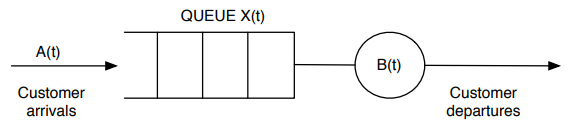
\includegraphics[width=6cm]{img_17.png}
\end{figure}
\begin{figure}[H]
\centering
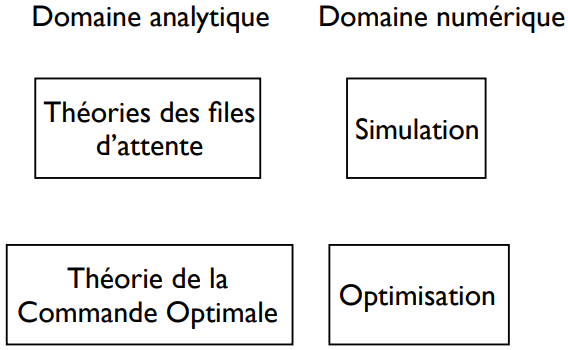
\includegraphics[width=6.00cm]{img_18.png}
\end{figure}
\begin{center}
\small
\begin{tabular}{ll}
Temps inter-arrivée & $Y_k$\\
Taux moyen d'arrivée (fréquence) & $\lambda$\\
Temps moyen inter-arrivée & $E[Y]=1/\lambda$\\
Temps de service & $Z_k$\\
Fréquence moyenne de service & $\mu$\\
Moyenne des temps de service & $E[Z]=1/\mu$\\
Capacité de stockage (parfois $\infty$) & $K$\\
Nombre de serveurs & $m$\\
Temps d'arrivée & $A_k$\\
Temps de départ & $D_k$\\
Temps d'attente & $W_k$\\
Temps de système & $S_k$\\
Longueur de file & $X(t)$\\
Charge & $U(t)$\\
Temps moyen d'attente (régime établi) & $E[W]$\\
Temps de service moyen (régime établi) & $E[Z]$\\
Nombre moyen de clients (régime établi) & $E[X]$\\
Charge de travail moyenne (rég. établi) & $E[U]$
\end{tabular}
\end{center}
\paragraph{Notation} $A/B/m/K$
\subsection{Relations}
$$S_k=D_k-A_k=W_k+Z_k$$
$$D_k=A_k+W_k+Z_k$$
\subsection{Temps moyen d'attente et de service}
si $k\to\infty$ il peut y avoir une distribution stationnaire
\subsection{Optimisation}
On veut :
\begin{itemize}
\item Minimiser le temps d'attente
\item Maximiser l'utilisation du serveur
\end{itemize}
Donc minimiser $E[W]$, $E[Z]$ et $E[X]$. On veut maximiser l'utilisation et le débit
\subsection{Intensité du trafic}
$$\text{intensité du trafic} = \frac{\text{fréquence d'arrivée}}{\text{fréquence de sortie}}$$
$$\rho=\frac{\lambda}{m\mu}=(1-\pi_0)$$
\subsection{Utilisation et throughput}
$\pi_0$ probabilité que la file soit vide (fraction du temps pendant laquelle le serveur est inutilisé)
$$\text{throughput} = \text{taux de départ des clients} = \mu(1-\pi_0)$$
En régime permanent :
$$\lambda=\mu(1-\pi_0)$$
\subsection{Équation de Lindley}
$$W_k=\max\lbrace 0,W_{k-1}+Z_{k-1}-Y_k\rbrace$$
$$D_k=\max\lbrace A_k,D_{k-1}\rbrace +Z_k$$
\subsection{Loi de Little}
\begin{center}
\begin{tabular}{p{5cm}l}
Nombre d'arrivées de clients jusqu'au temps $t$ & $n_a(t)$\\
Nombre de départs de clients jusqu'au temps $t$ & $n_d(t)$\\
Nombre de clients dans le système au temps $t$ & $X(t)$\\
\end{tabular}
\end{center}
$$X(t)=n_a(t)-n_d(t)$$
\subsubsection{Dérivation}
Temps moyen dans le système / client
$$\bar{s}(t)=\frac{u(t)}{n_a(t)}$$
Nombre moyen de clients dans le système
$$\bar{x}(t)=\frac{u(t)}{t}$$
Fréquence moyenne d'arrivée
$$\lambda(t)=\frac{n_a(t)}{t}$$
$$\bar{x}(t)=\lambda(t)\bar{s}(t)$$
Taux moyen d'arrivée en régime établi :
$$\lim_{t\to\infty}\lambda(t)=\lambda$$
Temps moyen du système en régime établi :
$$\lim_{t\to\infty}\bar{s}(t)=s$$
$$\bar{x}=E[X]\qquad \bar{s}=E[S]$$
\subsection{Systèmes à file d'attente markoviens simples}
En régime établi :
$$\lambda=\mu(1-\pi_0)\qquad \rho(1-\pi_0)$$
\begin{figure}[H]
\centering
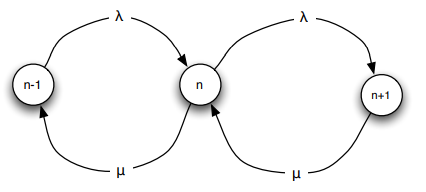
\includegraphics[width=6.00cm]{img_19.png}
\end{figure}
Probabilité d'aller de l'état $n-1$ à $n$
$$\lambda\pi_{n-1}$$
Probabilité d'aller de l'état $n$ à $n-1$
$$\mu\pi_n$$
Probabilité d'avoir $n$ clients dans le système
$$\pi_n=\rho^{n}\pi_0=(1-\rho)\rho^n$$
Équation de récurrence
$$\pi_n=\rho\pi_{n-1}$$





\end{document}